% Options for packages loaded elsewhere
\PassOptionsToPackage{unicode}{hyperref}
\PassOptionsToPackage{hyphens}{url}
\PassOptionsToPackage{dvipsnames,svgnames,x11names}{xcolor}
%
\documentclass[
  letterpaper,
  DIV=11,
  numbers=noendperiod]{scrartcl}

\usepackage{amsmath,amssymb}
\usepackage{iftex}
\ifPDFTeX
  \usepackage[T1]{fontenc}
  \usepackage[utf8]{inputenc}
  \usepackage{textcomp} % provide euro and other symbols
\else % if luatex or xetex
  \usepackage{unicode-math}
  \defaultfontfeatures{Scale=MatchLowercase}
  \defaultfontfeatures[\rmfamily]{Ligatures=TeX,Scale=1}
\fi
\usepackage{lmodern}
\ifPDFTeX\else  
    % xetex/luatex font selection
\fi
% Use upquote if available, for straight quotes in verbatim environments
\IfFileExists{upquote.sty}{\usepackage{upquote}}{}
\IfFileExists{microtype.sty}{% use microtype if available
  \usepackage[]{microtype}
  \UseMicrotypeSet[protrusion]{basicmath} % disable protrusion for tt fonts
}{}
\makeatletter
\@ifundefined{KOMAClassName}{% if non-KOMA class
  \IfFileExists{parskip.sty}{%
    \usepackage{parskip}
  }{% else
    \setlength{\parindent}{0pt}
    \setlength{\parskip}{6pt plus 2pt minus 1pt}}
}{% if KOMA class
  \KOMAoptions{parskip=half}}
\makeatother
\usepackage{xcolor}
\setlength{\emergencystretch}{3em} % prevent overfull lines
\setcounter{secnumdepth}{-\maxdimen} % remove section numbering
% Make \paragraph and \subparagraph free-standing
\makeatletter
\ifx\paragraph\undefined\else
  \let\oldparagraph\paragraph
  \renewcommand{\paragraph}{
    \@ifstar
      \xxxParagraphStar
      \xxxParagraphNoStar
  }
  \newcommand{\xxxParagraphStar}[1]{\oldparagraph*{#1}\mbox{}}
  \newcommand{\xxxParagraphNoStar}[1]{\oldparagraph{#1}\mbox{}}
\fi
\ifx\subparagraph\undefined\else
  \let\oldsubparagraph\subparagraph
  \renewcommand{\subparagraph}{
    \@ifstar
      \xxxSubParagraphStar
      \xxxSubParagraphNoStar
  }
  \newcommand{\xxxSubParagraphStar}[1]{\oldsubparagraph*{#1}\mbox{}}
  \newcommand{\xxxSubParagraphNoStar}[1]{\oldsubparagraph{#1}\mbox{}}
\fi
\makeatother

\usepackage{color}
\usepackage{fancyvrb}
\newcommand{\VerbBar}{|}
\newcommand{\VERB}{\Verb[commandchars=\\\{\}]}
\DefineVerbatimEnvironment{Highlighting}{Verbatim}{commandchars=\\\{\}}
% Add ',fontsize=\small' for more characters per line
\usepackage{framed}
\definecolor{shadecolor}{RGB}{241,243,245}
\newenvironment{Shaded}{\begin{snugshade}}{\end{snugshade}}
\newcommand{\AlertTok}[1]{\textcolor[rgb]{0.68,0.00,0.00}{#1}}
\newcommand{\AnnotationTok}[1]{\textcolor[rgb]{0.37,0.37,0.37}{#1}}
\newcommand{\AttributeTok}[1]{\textcolor[rgb]{0.40,0.45,0.13}{#1}}
\newcommand{\BaseNTok}[1]{\textcolor[rgb]{0.68,0.00,0.00}{#1}}
\newcommand{\BuiltInTok}[1]{\textcolor[rgb]{0.00,0.23,0.31}{#1}}
\newcommand{\CharTok}[1]{\textcolor[rgb]{0.13,0.47,0.30}{#1}}
\newcommand{\CommentTok}[1]{\textcolor[rgb]{0.37,0.37,0.37}{#1}}
\newcommand{\CommentVarTok}[1]{\textcolor[rgb]{0.37,0.37,0.37}{\textit{#1}}}
\newcommand{\ConstantTok}[1]{\textcolor[rgb]{0.56,0.35,0.01}{#1}}
\newcommand{\ControlFlowTok}[1]{\textcolor[rgb]{0.00,0.23,0.31}{\textbf{#1}}}
\newcommand{\DataTypeTok}[1]{\textcolor[rgb]{0.68,0.00,0.00}{#1}}
\newcommand{\DecValTok}[1]{\textcolor[rgb]{0.68,0.00,0.00}{#1}}
\newcommand{\DocumentationTok}[1]{\textcolor[rgb]{0.37,0.37,0.37}{\textit{#1}}}
\newcommand{\ErrorTok}[1]{\textcolor[rgb]{0.68,0.00,0.00}{#1}}
\newcommand{\ExtensionTok}[1]{\textcolor[rgb]{0.00,0.23,0.31}{#1}}
\newcommand{\FloatTok}[1]{\textcolor[rgb]{0.68,0.00,0.00}{#1}}
\newcommand{\FunctionTok}[1]{\textcolor[rgb]{0.28,0.35,0.67}{#1}}
\newcommand{\ImportTok}[1]{\textcolor[rgb]{0.00,0.46,0.62}{#1}}
\newcommand{\InformationTok}[1]{\textcolor[rgb]{0.37,0.37,0.37}{#1}}
\newcommand{\KeywordTok}[1]{\textcolor[rgb]{0.00,0.23,0.31}{\textbf{#1}}}
\newcommand{\NormalTok}[1]{\textcolor[rgb]{0.00,0.23,0.31}{#1}}
\newcommand{\OperatorTok}[1]{\textcolor[rgb]{0.37,0.37,0.37}{#1}}
\newcommand{\OtherTok}[1]{\textcolor[rgb]{0.00,0.23,0.31}{#1}}
\newcommand{\PreprocessorTok}[1]{\textcolor[rgb]{0.68,0.00,0.00}{#1}}
\newcommand{\RegionMarkerTok}[1]{\textcolor[rgb]{0.00,0.23,0.31}{#1}}
\newcommand{\SpecialCharTok}[1]{\textcolor[rgb]{0.37,0.37,0.37}{#1}}
\newcommand{\SpecialStringTok}[1]{\textcolor[rgb]{0.13,0.47,0.30}{#1}}
\newcommand{\StringTok}[1]{\textcolor[rgb]{0.13,0.47,0.30}{#1}}
\newcommand{\VariableTok}[1]{\textcolor[rgb]{0.07,0.07,0.07}{#1}}
\newcommand{\VerbatimStringTok}[1]{\textcolor[rgb]{0.13,0.47,0.30}{#1}}
\newcommand{\WarningTok}[1]{\textcolor[rgb]{0.37,0.37,0.37}{\textit{#1}}}

\providecommand{\tightlist}{%
  \setlength{\itemsep}{0pt}\setlength{\parskip}{0pt}}\usepackage{longtable,booktabs,array}
\usepackage{calc} % for calculating minipage widths
% Correct order of tables after \paragraph or \subparagraph
\usepackage{etoolbox}
\makeatletter
\patchcmd\longtable{\par}{\if@noskipsec\mbox{}\fi\par}{}{}
\makeatother
% Allow footnotes in longtable head/foot
\IfFileExists{footnotehyper.sty}{\usepackage{footnotehyper}}{\usepackage{footnote}}
\makesavenoteenv{longtable}
\usepackage{graphicx}
\makeatletter
\def\maxwidth{\ifdim\Gin@nat@width>\linewidth\linewidth\else\Gin@nat@width\fi}
\def\maxheight{\ifdim\Gin@nat@height>\textheight\textheight\else\Gin@nat@height\fi}
\makeatother
% Scale images if necessary, so that they will not overflow the page
% margins by default, and it is still possible to overwrite the defaults
% using explicit options in \includegraphics[width, height, ...]{}
\setkeys{Gin}{width=\maxwidth,height=\maxheight,keepaspectratio}
% Set default figure placement to htbp
\makeatletter
\def\fps@figure{htbp}
\makeatother

\KOMAoption{captions}{tableheading}
\makeatletter
\@ifpackageloaded{caption}{}{\usepackage{caption}}
\AtBeginDocument{%
\ifdefined\contentsname
  \renewcommand*\contentsname{Table of contents}
\else
  \newcommand\contentsname{Table of contents}
\fi
\ifdefined\listfigurename
  \renewcommand*\listfigurename{List of Figures}
\else
  \newcommand\listfigurename{List of Figures}
\fi
\ifdefined\listtablename
  \renewcommand*\listtablename{List of Tables}
\else
  \newcommand\listtablename{List of Tables}
\fi
\ifdefined\figurename
  \renewcommand*\figurename{Figure}
\else
  \newcommand\figurename{Figure}
\fi
\ifdefined\tablename
  \renewcommand*\tablename{Table}
\else
  \newcommand\tablename{Table}
\fi
}
\@ifpackageloaded{float}{}{\usepackage{float}}
\floatstyle{ruled}
\@ifundefined{c@chapter}{\newfloat{codelisting}{h}{lop}}{\newfloat{codelisting}{h}{lop}[chapter]}
\floatname{codelisting}{Listing}
\newcommand*\listoflistings{\listof{codelisting}{List of Listings}}
\makeatother
\makeatletter
\makeatother
\makeatletter
\@ifpackageloaded{caption}{}{\usepackage{caption}}
\@ifpackageloaded{subcaption}{}{\usepackage{subcaption}}
\makeatother

\ifLuaTeX
  \usepackage{selnolig}  % disable illegal ligatures
\fi
\usepackage{bookmark}

\IfFileExists{xurl.sty}{\usepackage{xurl}}{} % add URL line breaks if available
\urlstyle{same} % disable monospaced font for URLs
\hypersetup{
  pdftitle={class 10: Structure Bioinformatics 1},
  pdfauthor={Vivian Bach (PID:A18497911)},
  colorlinks=true,
  linkcolor={blue},
  filecolor={Maroon},
  citecolor={Blue},
  urlcolor={Blue},
  pdfcreator={LaTeX via pandoc}}


\title{class 10: Structure Bioinformatics 1}
\author{Vivian Bach (PID:A18497911)}
\date{}

\begin{document}
\maketitle


\subsection{PDB Statistics}\label{pdb-statistics}

The protien Data Bank (PDB) is the main respositry biomolecular
structures. Let's see what it contains:

\begin{Shaded}
\begin{Highlighting}[]
\FunctionTok{library}\NormalTok{(readr)}
\NormalTok{stats }\OtherTok{\textless{}{-}} \FunctionTok{read.csv}\NormalTok{(}\StringTok{"Data Export Summary.csv"}\NormalTok{)}
\NormalTok{stats}
\end{Highlighting}
\end{Shaded}

\begin{verbatim}
           Molecular.Type   X.ray     EM    NMR Integrative Multiple.methods
1          Protein (only) 178,795 21,825 12,773         343              226
2 Protein/Oligosaccharide  10,363  3,564     34           8               11
3              Protein/NA   9,106  6,335    287          24                7
4     Nucleic acid (only)   3,132    221  1,566           3               15
5                   Other     175     25     33           4                0
6  Oligosaccharide (only)      11      0      6           0                1
  Neutron Other   Total
1      84    32 214,078
2       1     0  13,981
3       0     0  15,759
4       3     1   4,941
5       0     0     237
6       0     4      22
\end{verbatim}

The comma in these numbers leads to the numbers being read as character.

\begin{Shaded}
\begin{Highlighting}[]
\FunctionTok{c}\NormalTok{(}\DecValTok{100}\NormalTok{,}\DecValTok{10}\NormalTok{,}\StringTok{""}\NormalTok{)}
\end{Highlighting}
\end{Shaded}

\begin{verbatim}
[1] "100" "10"  ""   
\end{verbatim}

\begin{Shaded}
\begin{Highlighting}[]
\FunctionTok{library}\NormalTok{(readr)}
\NormalTok{stats }\OtherTok{\textless{}{-}} \FunctionTok{read\_csv}\NormalTok{(}\StringTok{"Data Export Summary.csv"}\NormalTok{)}
\end{Highlighting}
\end{Shaded}

\begin{verbatim}
Rows: 6 Columns: 9
-- Column specification --------------------------------------------------------
Delimiter: ","
chr (1): Molecular Type
dbl (4): Integrative, Multiple methods, Neutron, Other
num (4): X-ray, EM, NMR, Total

i Use `spec()` to retrieve the full column specification for this data.
i Specify the column types or set `show_col_types = FALSE` to quiet this message.
\end{verbatim}

\begin{Shaded}
\begin{Highlighting}[]
\NormalTok{stats}
\end{Highlighting}
\end{Shaded}

\begin{verbatim}
# A tibble: 6 x 9
  `Molecular Type`    `X-ray`    EM   NMR Integrative `Multiple methods` Neutron
  <chr>                 <dbl> <dbl> <dbl>       <dbl>              <dbl>   <dbl>
1 Protein (only)       178795 21825 12773         343                226      84
2 Protein/Oligosacch~   10363  3564    34           8                 11       1
3 Protein/NA             9106  6335   287          24                  7       0
4 Nucleic acid (only)    3132   221  1566           3                 15       3
5 Other                   175    25    33           4                  0       0
6 Oligosaccharide (o~      11     0     6           0                  1       0
# i 2 more variables: Other <dbl>, Total <dbl>
\end{verbatim}

\begin{Shaded}
\begin{Highlighting}[]
\FunctionTok{sum}\NormalTok{(}\FunctionTok{c}\NormalTok{(stats}\SpecialCharTok{$}\StringTok{\textasciigrave{}}\AttributeTok{X{-}ray}\StringTok{\textasciigrave{}}\NormalTok{, stats}\SpecialCharTok{$}\StringTok{\textasciigrave{}}\AttributeTok{EM}\StringTok{\textasciigrave{}}\NormalTok{))}
\end{Highlighting}
\end{Shaded}

\begin{verbatim}
[1] 233552
\end{verbatim}

\begin{quote}
Q1: What percentage of structures in the PDB are solved by X-Ray and
Electron Microscopy
\end{quote}

\begin{Shaded}
\begin{Highlighting}[]
\NormalTok{n.xray }\OtherTok{\textless{}{-}} \FunctionTok{sum}\NormalTok{(stats}\SpecialCharTok{$}\StringTok{\textasciigrave{}}\AttributeTok{X{-}ray}\StringTok{\textasciigrave{}}\NormalTok{)}
\CommentTok{\#n.em \textless{}{-}}
\NormalTok{n.total }\OtherTok{\textless{}{-}} \FunctionTok{sum}\NormalTok{(stats}\SpecialCharTok{$}\NormalTok{Total)}

\NormalTok{n.xray}\SpecialCharTok{/}\NormalTok{n.total}
\end{Highlighting}
\end{Shaded}

\begin{verbatim}
[1] 0.8095077
\end{verbatim}

\begin{quote}
Q2: What proportion of structures in the PDB are protein?
\end{quote}

\begin{Shaded}
\begin{Highlighting}[]
\NormalTok{n.protein }\OtherTok{\textless{}{-}}\NormalTok{ stats[}\DecValTok{1}\NormalTok{, }\StringTok{"Total"}\NormalTok{]}
\NormalTok{p\_protein }\OtherTok{\textless{}{-}}\NormalTok{ n.protein}\SpecialCharTok{/}\NormalTok{n.total}
\NormalTok{p\_protein}
\end{Highlighting}
\end{Shaded}

\begin{verbatim}
      Total
1 0.8596889
\end{verbatim}

\begin{quote}
Q3: Skip
\end{quote}

\subsection{Visualizing the HIV-1 protease
structure}\label{visualizing-the-hiv-1-protease-structure}

We can use the Molstar viewer online: https://molstar.org/viewer/

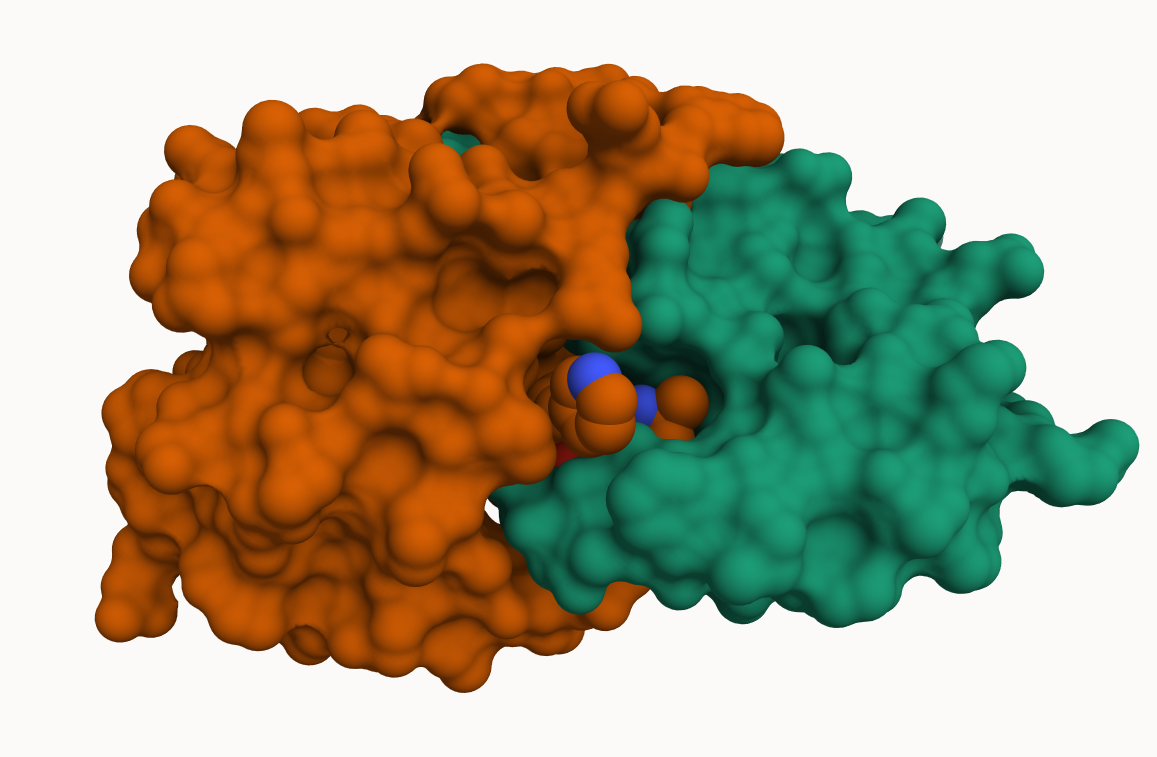
\includegraphics{1HSG.png} A clean image showing the catalytic ASP25
amino acids in both chains of the HIV-PR dimer along with the inhibitor
and all important active site water.

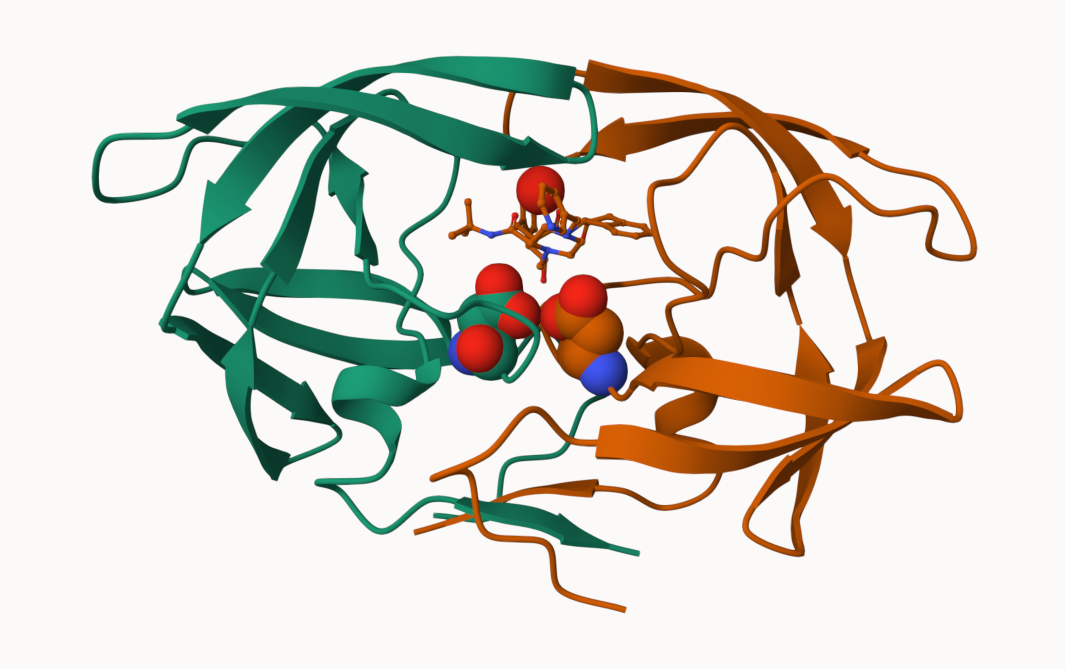
\includegraphics{1HSG_2.png} \#\# Bio3D package for structural
bioinformatics

\begin{Shaded}
\begin{Highlighting}[]
\FunctionTok{library}\NormalTok{(bio3d)}
\NormalTok{pdb }\OtherTok{\textless{}{-}} \FunctionTok{read.pdb}\NormalTok{(}\StringTok{"1hsg"}\NormalTok{)}
\end{Highlighting}
\end{Shaded}

\begin{verbatim}
  Note: Accessing on-line PDB file
\end{verbatim}

\begin{Shaded}
\begin{Highlighting}[]
\NormalTok{pdb}
\end{Highlighting}
\end{Shaded}

\begin{verbatim}

 Call:  read.pdb(file = "1hsg")

   Total Models#: 1
     Total Atoms#: 1686,  XYZs#: 5058  Chains#: 2  (values: A B)

     Protein Atoms#: 1514  (residues/Calpha atoms#: 198)
     Nucleic acid Atoms#: 0  (residues/phosphate atoms#: 0)

     Non-protein/nucleic Atoms#: 172  (residues: 128)
     Non-protein/nucleic resid values: [ HOH (127), MK1 (1) ]

   Protein sequence:
      PQITLWQRPLVTIKIGGQLKEALLDTGADDTVLEEMSLPGRWKPKMIGGIGGFIKVRQYD
      QILIEICGHKAIGTVLVGPTPVNIIGRNLLTQIGCTLNFPQITLWQRPLVTIKIGGQLKE
      ALLDTGADDTVLEEMSLPGRWKPKMIGGIGGFIKVRQYDQILIEICGHKAIGTVLVGPTP
      VNIIGRNLLTQIGCTLNF

+ attr: atom, xyz, seqres, helix, sheet,
        calpha, remark, call
\end{verbatim}

\begin{Shaded}
\begin{Highlighting}[]
\FunctionTok{head}\NormalTok{(pdb}\SpecialCharTok{$}\NormalTok{atom)}
\end{Highlighting}
\end{Shaded}

\begin{verbatim}
  type eleno elety  alt resid chain resno insert      x      y     z o     b
1 ATOM     1     N <NA>   PRO     A     1   <NA> 29.361 39.686 5.862 1 38.10
2 ATOM     2    CA <NA>   PRO     A     1   <NA> 30.307 38.663 5.319 1 40.62
3 ATOM     3     C <NA>   PRO     A     1   <NA> 29.760 38.071 4.022 1 42.64
4 ATOM     4     O <NA>   PRO     A     1   <NA> 28.600 38.302 3.676 1 43.40
5 ATOM     5    CB <NA>   PRO     A     1   <NA> 30.508 37.541 6.342 1 37.87
6 ATOM     6    CG <NA>   PRO     A     1   <NA> 29.296 37.591 7.162 1 38.40
  segid elesy charge
1  <NA>     N   <NA>
2  <NA>     C   <NA>
3  <NA>     C   <NA>
4  <NA>     O   <NA>
5  <NA>     C   <NA>
6  <NA>     C   <NA>
\end{verbatim}

\begin{Shaded}
\begin{Highlighting}[]
\CommentTok{\#library(bio3dview)}
\CommentTok{\#view.pdb(pdb)}
\CommentTok{\#was unable to install packages :(}
\end{Highlighting}
\end{Shaded}

\subsection{Predicting functional motions of a single
structure}\label{predicting-functional-motions-of-a-single-structure}

Read an ADK structure from the PDB database:

\begin{Shaded}
\begin{Highlighting}[]
\NormalTok{adk }\OtherTok{\textless{}{-}} \FunctionTok{read.pdb}\NormalTok{(}\StringTok{"6s36"}\NormalTok{)}
\end{Highlighting}
\end{Shaded}

\begin{verbatim}
  Note: Accessing on-line PDB file
   PDB has ALT records, taking A only, rm.alt=TRUE
\end{verbatim}

\begin{Shaded}
\begin{Highlighting}[]
\NormalTok{adk}
\end{Highlighting}
\end{Shaded}

\begin{verbatim}

 Call:  read.pdb(file = "6s36")

   Total Models#: 1
     Total Atoms#: 1898,  XYZs#: 5694  Chains#: 1  (values: A)

     Protein Atoms#: 1654  (residues/Calpha atoms#: 214)
     Nucleic acid Atoms#: 0  (residues/phosphate atoms#: 0)

     Non-protein/nucleic Atoms#: 244  (residues: 244)
     Non-protein/nucleic resid values: [ CL (3), HOH (238), MG (2), NA (1) ]

   Protein sequence:
      MRIILLGAPGAGKGTQAQFIMEKYGIPQISTGDMLRAAVKSGSELGKQAKDIMDAGKLVT
      DELVIALVKERIAQEDCRNGFLLDGFPRTIPQADAMKEAGINVDYVLEFDVPDELIVDKI
      VGRRVHAPSGRVYHVKFNPPKVEGKDDVTGEELTTRKDDQEETVRKRLVEYHQMTAPLIG
      YYSKEAEAGNTKYAKVDGTKPVAEVRADLEKILG

+ attr: atom, xyz, seqres, helix, sheet,
        calpha, remark, call
\end{verbatim}

\begin{Shaded}
\begin{Highlighting}[]
\NormalTok{m }\OtherTok{\textless{}{-}} \FunctionTok{nma}\NormalTok{(adk)}
\end{Highlighting}
\end{Shaded}

\begin{verbatim}
 Building Hessian...        Done in 0.01 seconds.
 Diagonalizing Hessian...   Done in 0.224 seconds.
\end{verbatim}

\begin{Shaded}
\begin{Highlighting}[]
\FunctionTok{plot}\NormalTok{(m)}
\end{Highlighting}
\end{Shaded}

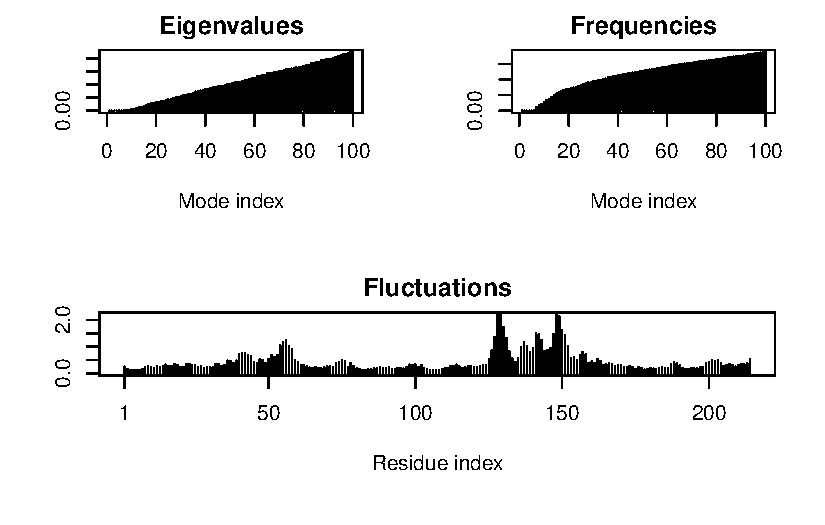
\includegraphics{Class-10_files/figure-pdf/unnamed-chunk-11-1.pdf}

Write out our results a wee trajectory/movie of predicted motion:

\begin{Shaded}
\begin{Highlighting}[]
\FunctionTok{mktrj}\NormalTok{(m, }\AttributeTok{file=}\StringTok{"adk\_m7.pdb"}\NormalTok{)}
\end{Highlighting}
\end{Shaded}

\subsection{comparative analysis with PCA
(2/10)}\label{comparative-analysis-with-pca-210}

First steo find an ADK sequence:

\begin{Shaded}
\begin{Highlighting}[]
\FunctionTok{library}\NormalTok{(bio3d)}
\NormalTok{id }\OtherTok{\textless{}{-}} \StringTok{"1ake\_A"} \DocumentationTok{\#\#change this to run a different analysis }
\NormalTok{aa }\OtherTok{\textless{}{-}}\FunctionTok{get.seq}\NormalTok{(id)}
\end{Highlighting}
\end{Shaded}

\begin{verbatim}
Warning in get.seq(id): Removing existing file: seqs.fasta
\end{verbatim}

\begin{verbatim}
Fetching... Please wait. Done.
\end{verbatim}

\begin{Shaded}
\begin{Highlighting}[]
\NormalTok{aa}
\end{Highlighting}
\end{Shaded}

\begin{verbatim}
             1        .         .         .         .         .         60 
pdb|1AKE|A   MRIILLGAPGAGKGTQAQFIMEKYGIPQISTGDMLRAAVKSGSELGKQAKDIMDAGKLVT
             1        .         .         .         .         .         60 

            61        .         .         .         .         .         120 
pdb|1AKE|A   DELVIALVKERIAQEDCRNGFLLDGFPRTIPQADAMKEAGINVDYVLEFDVPDELIVDRI
            61        .         .         .         .         .         120 

           121        .         .         .         .         .         180 
pdb|1AKE|A   VGRRVHAPSGRVYHVKFNPPKVEGKDDVTGEELTTRKDDQEETVRKRLVEYHQMTAPLIG
           121        .         .         .         .         .         180 

           181        .         .         .   214 
pdb|1AKE|A   YYSKEAEAGNTKYAKVDGTKPVAEVRADLEKILG
           181        .         .         .   214 

Call:
  read.fasta(file = outfile)

Class:
  fasta

Alignment dimensions:
  1 sequence rows; 214 position columns (214 non-gap, 0 gap) 

+ attr: id, ali, call
\end{verbatim}

Next step, is search the PDB database for all related entries

\begin{Shaded}
\begin{Highlighting}[]
\NormalTok{blast }\OtherTok{\textless{}{-}} \FunctionTok{blast.pdb}\NormalTok{(aa)}
\end{Highlighting}
\end{Shaded}

\begin{verbatim}
 Searching ... please wait (updates every 5 seconds) RID = SPXVT9ZP016 
 .
 Reporting 96 hits
\end{verbatim}

\begin{Shaded}
\begin{Highlighting}[]
\NormalTok{hits}\OtherTok{\textless{}{-}} \FunctionTok{plot}\NormalTok{(blast)}
\end{Highlighting}
\end{Shaded}

\begin{verbatim}
  * Possible cutoff values:    260 3 
            Yielding Nhits:    20 96 

  * Chosen cutoff value of:    260 
            Yielding Nhits:    20 
\end{verbatim}

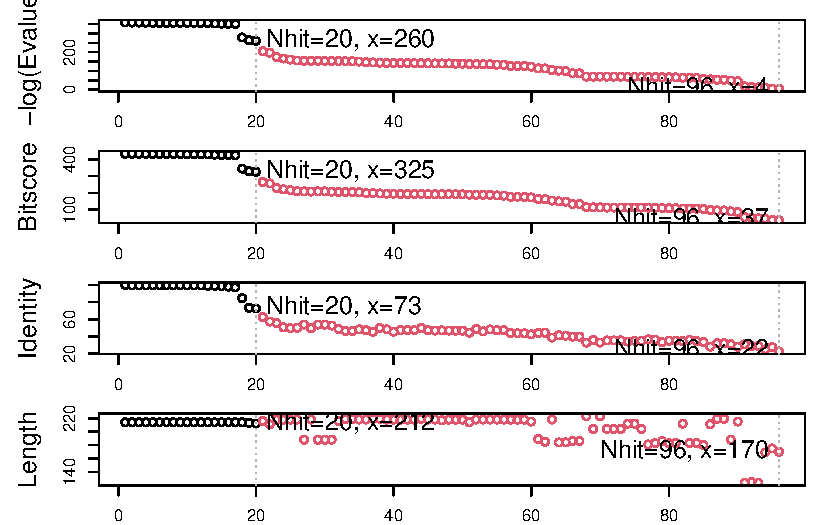
\includegraphics{Class-10_files/figure-pdf/unnamed-chunk-15-1.pdf}

All Blast results are heare for us to see

\begin{Shaded}
\begin{Highlighting}[]
\FunctionTok{head}\NormalTok{ (blast}\SpecialCharTok{$}\NormalTok{hit.tbl)}
\end{Highlighting}
\end{Shaded}

\begin{verbatim}
        queryid subjectids identity alignmentlength mismatches gapopens q.start
1 Query_5423451     1AKE_A  100.000             214          0        0       1
2 Query_5423451     8BQF_A   99.533             214          1        0       1
3 Query_5423451     4X8M_A   99.533             214          1        0       1
4 Query_5423451     6S36_A   99.533             214          1        0       1
5 Query_5423451     9R6U_A   99.533             214          1        0       1
6 Query_5423451     9R71_A   99.533             214          1        0       1
  q.end s.start s.end    evalue bitscore positives mlog.evalue pdb.id    acc
1   214       1   214 1.78e-156      432    100.00    358.6267 1AKE_A 1AKE_A
2   214      21   234 2.91e-156      433    100.00    358.1351 8BQF_A 8BQF_A
3   214       1   214 3.18e-156      432    100.00    358.0464 4X8M_A 4X8M_A
4   214       1   214 4.67e-156      432    100.00    357.6621 6S36_A 6S36_A
5   214       1   214 1.04e-155      431     99.53    356.8615 9R6U_A 9R6U_A
6   214       1   214 1.23e-155      431     99.53    356.6937 9R71_A 9R71_A
\end{verbatim}

The ``top hits'' are in their \texttt{hits} object. Now we can download
these to our computer. Put these in a wee sub-folder (directory) called
``pdbs'' and use gzip to speed things up

\begin{Shaded}
\begin{Highlighting}[]
\CommentTok{\# Download releated PDB files}
\NormalTok{files }\OtherTok{\textless{}{-}} \FunctionTok{get.pdb}\NormalTok{(hits}\SpecialCharTok{$}\NormalTok{pdb.id, }\AttributeTok{path=}\StringTok{"pdbs"}\NormalTok{, }\AttributeTok{split=}\ConstantTok{TRUE}\NormalTok{, }\AttributeTok{gzip=}\ConstantTok{TRUE}\NormalTok{)}
\end{Highlighting}
\end{Shaded}

\begin{verbatim}
Warning in get.pdb(hits$pdb.id, path = "pdbs", split = TRUE, gzip = TRUE):
pdbs/1AKE.pdb.gz exists. Skipping download
\end{verbatim}

\begin{verbatim}
Warning in get.pdb(hits$pdb.id, path = "pdbs", split = TRUE, gzip = TRUE):
pdbs/8BQF.pdb.gz exists. Skipping download
\end{verbatim}

\begin{verbatim}
Warning in get.pdb(hits$pdb.id, path = "pdbs", split = TRUE, gzip = TRUE):
pdbs/4X8M.pdb.gz exists. Skipping download
\end{verbatim}

\begin{verbatim}
Warning in get.pdb(hits$pdb.id, path = "pdbs", split = TRUE, gzip = TRUE):
pdbs/6S36.pdb.gz exists. Skipping download
\end{verbatim}

\begin{verbatim}
Warning in get.pdb(hits$pdb.id, path = "pdbs", split = TRUE, gzip = TRUE):
pdbs/9R6U.pdb.gz exists. Skipping download
\end{verbatim}

\begin{verbatim}
Warning in get.pdb(hits$pdb.id, path = "pdbs", split = TRUE, gzip = TRUE):
pdbs/9R71.pdb.gz exists. Skipping download
\end{verbatim}

\begin{verbatim}
Warning in get.pdb(hits$pdb.id, path = "pdbs", split = TRUE, gzip = TRUE):
pdbs/8Q2B.pdb.gz exists. Skipping download
\end{verbatim}

\begin{verbatim}
Warning in get.pdb(hits$pdb.id, path = "pdbs", split = TRUE, gzip = TRUE):
pdbs/8RJ9.pdb.gz exists. Skipping download
\end{verbatim}

\begin{verbatim}
Warning in get.pdb(hits$pdb.id, path = "pdbs", split = TRUE, gzip = TRUE):
pdbs/6RZE.pdb.gz exists. Skipping download
\end{verbatim}

\begin{verbatim}
Warning in get.pdb(hits$pdb.id, path = "pdbs", split = TRUE, gzip = TRUE):
pdbs/4X8H.pdb.gz exists. Skipping download
\end{verbatim}

\begin{verbatim}
Warning in get.pdb(hits$pdb.id, path = "pdbs", split = TRUE, gzip = TRUE):
pdbs/3HPR.pdb.gz exists. Skipping download
\end{verbatim}

\begin{verbatim}
Warning in get.pdb(hits$pdb.id, path = "pdbs", split = TRUE, gzip = TRUE):
pdbs/1E4V.pdb.gz exists. Skipping download
\end{verbatim}

\begin{verbatim}
Warning in get.pdb(hits$pdb.id, path = "pdbs", split = TRUE, gzip = TRUE):
pdbs/5EJE.pdb.gz exists. Skipping download
\end{verbatim}

\begin{verbatim}
Warning in get.pdb(hits$pdb.id, path = "pdbs", split = TRUE, gzip = TRUE):
pdbs/1E4Y.pdb.gz exists. Skipping download
\end{verbatim}

\begin{verbatim}
Warning in get.pdb(hits$pdb.id, path = "pdbs", split = TRUE, gzip = TRUE):
pdbs/3X2S.pdb.gz exists. Skipping download
\end{verbatim}

\begin{verbatim}
Warning in get.pdb(hits$pdb.id, path = "pdbs", split = TRUE, gzip = TRUE):
pdbs/6HAP.pdb.gz exists. Skipping download
\end{verbatim}

\begin{verbatim}
Warning in get.pdb(hits$pdb.id, path = "pdbs", split = TRUE, gzip = TRUE):
pdbs/6HAM.pdb.gz exists. Skipping download
\end{verbatim}

\begin{verbatim}
Warning in get.pdb(hits$pdb.id, path = "pdbs", split = TRUE, gzip = TRUE):
pdbs/8PVW.pdb.gz exists. Skipping download
\end{verbatim}

\begin{verbatim}
Warning in get.pdb(hits$pdb.id, path = "pdbs", split = TRUE, gzip = TRUE):
pdbs/4K46.pdb.gz exists. Skipping download
\end{verbatim}

\begin{verbatim}
Warning in get.pdb(hits$pdb.id, path = "pdbs", split = TRUE, gzip = TRUE):
pdbs/4NP6.pdb.gz exists. Skipping download
\end{verbatim}

\begin{verbatim}

  |                                                                            
  |                                                                      |   0%
  |                                                                            
  |====                                                                  |   5%
  |                                                                            
  |=======                                                               |  10%
  |                                                                            
  |==========                                                            |  15%
  |                                                                            
  |==============                                                        |  20%
  |                                                                            
  |==================                                                    |  25%
  |                                                                            
  |=====================                                                 |  30%
  |                                                                            
  |========================                                              |  35%
  |                                                                            
  |============================                                          |  40%
  |                                                                            
  |================================                                      |  45%
  |                                                                            
  |===================================                                   |  50%
  |                                                                            
  |======================================                                |  55%
  |                                                                            
  |==========================================                            |  60%
  |                                                                            
  |==============================================                        |  65%
  |                                                                            
  |=================================================                     |  70%
  |                                                                            
  |====================================================                  |  75%
  |                                                                            
  |========================================================              |  80%
  |                                                                            
  |============================================================          |  85%
  |                                                                            
  |===============================================================       |  90%
  |                                                                            
  |==================================================================    |  95%
  |                                                                            
  |======================================================================| 100%
\end{verbatim}

These look like a hot mess

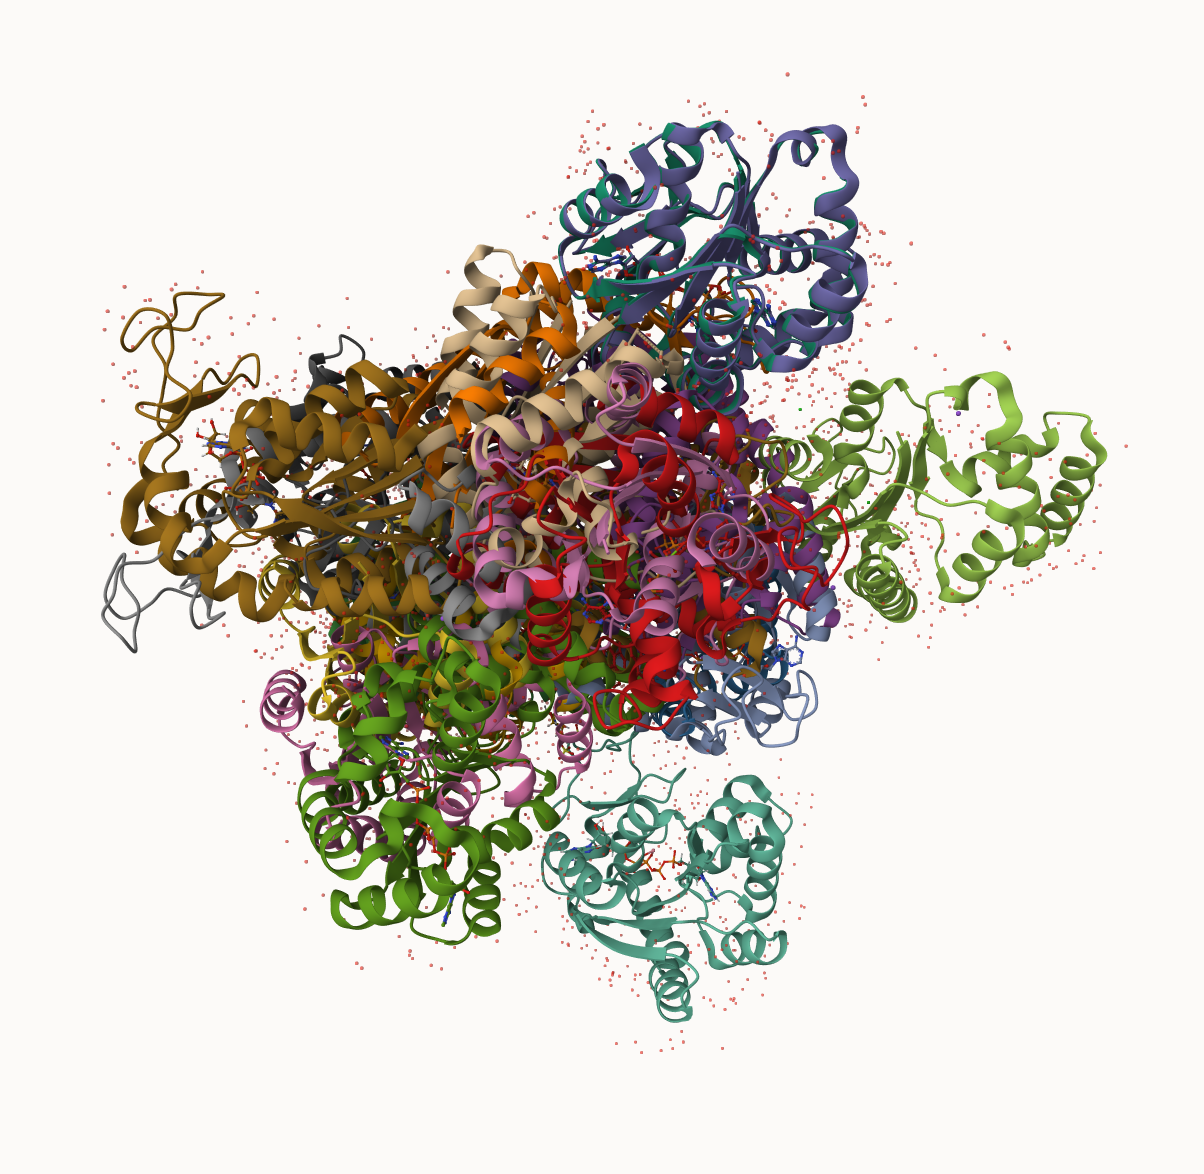
\includegraphics{1AKE-1E4V-1E4Y-3HPR-3X2S-4K46-4NP6-4X8H-4X8M-5EJE-6HAM-6HAP-6RZE-6S36-8BQF-8PVW-8Q2B-8RJ9-9R6U-9R71.png}
Next we will use the \texttt{pdbaln()} function to align and also
optionally fit (i.e.~suprepose) the identiified PDB structures.

This requires a BioConductor package called ``msa'' that we need to
install. First we install BiocManager. Then we use
\texttt{BiocManager::install("msa")}

\begin{Shaded}
\begin{Highlighting}[]
\CommentTok{\# Align releated PDBs}
\NormalTok{pdbs }\OtherTok{\textless{}{-}} \FunctionTok{pdbaln}\NormalTok{(files, }\AttributeTok{fit =} \ConstantTok{TRUE}\NormalTok{, }\AttributeTok{exefile=}\StringTok{"msa"}\NormalTok{)}
\end{Highlighting}
\end{Shaded}

\begin{verbatim}
Reading PDB files:
pdbs/split_chain/1AKE_A.pdb
pdbs/split_chain/8BQF_A.pdb
pdbs/split_chain/4X8M_A.pdb
pdbs/split_chain/6S36_A.pdb
pdbs/split_chain/9R6U_A.pdb
pdbs/split_chain/9R71_A.pdb
pdbs/split_chain/8Q2B_A.pdb
pdbs/split_chain/8RJ9_A.pdb
pdbs/split_chain/6RZE_A.pdb
pdbs/split_chain/4X8H_A.pdb
pdbs/split_chain/3HPR_A.pdb
pdbs/split_chain/1E4V_A.pdb
pdbs/split_chain/5EJE_A.pdb
pdbs/split_chain/1E4Y_A.pdb
pdbs/split_chain/3X2S_A.pdb
pdbs/split_chain/6HAP_A.pdb
pdbs/split_chain/6HAM_A.pdb
pdbs/split_chain/8PVW_A.pdb
pdbs/split_chain/4K46_A.pdb
pdbs/split_chain/4NP6_A.pdb
   PDB has ALT records, taking A only, rm.alt=TRUE
.   PDB has ALT records, taking A only, rm.alt=TRUE
..   PDB has ALT records, taking A only, rm.alt=TRUE
.   PDB has ALT records, taking A only, rm.alt=TRUE
.   PDB has ALT records, taking A only, rm.alt=TRUE
.   PDB has ALT records, taking A only, rm.alt=TRUE
.   PDB has ALT records, taking A only, rm.alt=TRUE
.   PDB has ALT records, taking A only, rm.alt=TRUE
..   PDB has ALT records, taking A only, rm.alt=TRUE
..   PDB has ALT records, taking A only, rm.alt=TRUE
....   PDB has ALT records, taking A only, rm.alt=TRUE
.   PDB has ALT records, taking A only, rm.alt=TRUE
.   PDB has ALT records, taking A only, rm.alt=TRUE
..

Extracting sequences

pdb/seq: 1   name: pdbs/split_chain/1AKE_A.pdb 
   PDB has ALT records, taking A only, rm.alt=TRUE
pdb/seq: 2   name: pdbs/split_chain/8BQF_A.pdb 
   PDB has ALT records, taking A only, rm.alt=TRUE
pdb/seq: 3   name: pdbs/split_chain/4X8M_A.pdb 
pdb/seq: 4   name: pdbs/split_chain/6S36_A.pdb 
   PDB has ALT records, taking A only, rm.alt=TRUE
pdb/seq: 5   name: pdbs/split_chain/9R6U_A.pdb 
   PDB has ALT records, taking A only, rm.alt=TRUE
pdb/seq: 6   name: pdbs/split_chain/9R71_A.pdb 
   PDB has ALT records, taking A only, rm.alt=TRUE
pdb/seq: 7   name: pdbs/split_chain/8Q2B_A.pdb 
   PDB has ALT records, taking A only, rm.alt=TRUE
pdb/seq: 8   name: pdbs/split_chain/8RJ9_A.pdb 
   PDB has ALT records, taking A only, rm.alt=TRUE
pdb/seq: 9   name: pdbs/split_chain/6RZE_A.pdb 
   PDB has ALT records, taking A only, rm.alt=TRUE
pdb/seq: 10   name: pdbs/split_chain/4X8H_A.pdb 
pdb/seq: 11   name: pdbs/split_chain/3HPR_A.pdb 
   PDB has ALT records, taking A only, rm.alt=TRUE
pdb/seq: 12   name: pdbs/split_chain/1E4V_A.pdb 
pdb/seq: 13   name: pdbs/split_chain/5EJE_A.pdb 
   PDB has ALT records, taking A only, rm.alt=TRUE
pdb/seq: 14   name: pdbs/split_chain/1E4Y_A.pdb 
pdb/seq: 15   name: pdbs/split_chain/3X2S_A.pdb 
pdb/seq: 16   name: pdbs/split_chain/6HAP_A.pdb 
pdb/seq: 17   name: pdbs/split_chain/6HAM_A.pdb 
   PDB has ALT records, taking A only, rm.alt=TRUE
pdb/seq: 18   name: pdbs/split_chain/8PVW_A.pdb 
   PDB has ALT records, taking A only, rm.alt=TRUE
pdb/seq: 19   name: pdbs/split_chain/4K46_A.pdb 
   PDB has ALT records, taking A only, rm.alt=TRUE
pdb/seq: 20   name: pdbs/split_chain/4NP6_A.pdb 
\end{verbatim}

Have a wee peak at this new ``alignment object'' \texttt{pdbs}

\begin{Shaded}
\begin{Highlighting}[]
\NormalTok{pdbs}
\end{Highlighting}
\end{Shaded}

\begin{verbatim}
                                1        .         .         .         40 
[Truncated_Name:1]1AKE_A.pdb    --MRIILLGAPGAGKGTQAQFIMEKYGIPQISTGDMLRAA
[Truncated_Name:2]8BQF_A.pdb    --MRIILLGAPGAGKGTQAQFIMEKYGIPQISTGDMLRAA
[Truncated_Name:3]4X8M_A.pdb    --MRIILLGAPGAGKGTQAQFIMEKYGIPQISTGDMLRAA
[Truncated_Name:4]6S36_A.pdb    --MRIILLGAPGAGKGTQAQFIMEKYGIPQISTGDMLRAA
[Truncated_Name:5]9R6U_A.pdb    --MRIILLGAPGAGKGTQAQFIMEKYGIPQISTGDMLRAA
[Truncated_Name:6]9R71_A.pdb    --MRIILLGAPGAGKGTQAQFIMEKYGIPQISTGDMLRAA
[Truncated_Name:7]8Q2B_A.pdb    --MRIILLGAPGAGKGTQAQFIMEKYGIPQISTGDMLRAA
[Truncated_Name:8]8RJ9_A.pdb    --MRIILLGAPGAGKGTQAQFIMEKYGIPQISTGDMLRAA
[Truncated_Name:9]6RZE_A.pdb    --MRIILLGAPGAGKGTQAQFIMEKYGIPQISTGDMLRAA
[Truncated_Name:10]4X8H_A.pdb   --MRIILLGAPGAGKGTQAQFIMEKYGIPQISTGDMLRAA
[Truncated_Name:11]3HPR_A.pdb   --MRIILLGAPGAGKGTQAQFIMEKYGIPQISTGDMLRAA
[Truncated_Name:12]1E4V_A.pdb   --MRIILLGAPVAGKGTQAQFIMEKYGIPQISTGDMLRAA
[Truncated_Name:13]5EJE_A.pdb   --MRIILLGAPGAGKGTQAQFIMEKYGIPQISTGDMLRAA
[Truncated_Name:14]1E4Y_A.pdb   --MRIILLGALVAGKGTQAQFIMEKYGIPQISTGDMLRAA
[Truncated_Name:15]3X2S_A.pdb   --MRIILLGAPGAGKGTQAQFIMEKYGIPQISTGDMLRAA
[Truncated_Name:16]6HAP_A.pdb   --MRIILLGAPGAGKGTQAQFIMEKYGIPQISTGDMLRAA
[Truncated_Name:17]6HAM_A.pdb   --MRIILLGAPGAGKGTQAQFIMEKYGIPQISTGDMLRAA
[Truncated_Name:18]8PVW_A.pdb   --MRIILLGAPGAGKGTQAQFIMEKYGIPQISTGDMLRAA
[Truncated_Name:19]4K46_A.pdb   --MRIILLGAPGAGKGTQAQFIMAKFGIPQISTGDMLRAA
[Truncated_Name:20]4NP6_A.pdb   NAMRIILLGAPGAGKGTQAQFIMEKFGIPQISTGDMLRAA
                                  ********  *********** *^************** 
                                1        .         .         .         40 

                               41        .         .         .         80 
[Truncated_Name:1]1AKE_A.pdb    VKSGSELGKQAKDIMDAGKLVTDELVIALVKERIAQEDCR
[Truncated_Name:2]8BQF_A.pdb    VKSGSELGKQAKDIMDAGKLVTDELVIALVKERIAQE---
[Truncated_Name:3]4X8M_A.pdb    VKSGSELGKQAKDIMDAGKLVTDELVIALVKERIAQEDCR
[Truncated_Name:4]6S36_A.pdb    VKSGSELGKQAKDIMDAGKLVTDELVIALVKERIAQEDCR
[Truncated_Name:5]9R6U_A.pdb    VKSGSELGAQAKDIMDAGKLVTDELVIALVKERIAQEDCR
[Truncated_Name:6]9R71_A.pdb    VKSGSELGKQAKDIMDAGKLVTDELVIALVKERIAQEDCR
[Truncated_Name:7]8Q2B_A.pdb    VKSGSELGKQAKDIMDAGKLVTDELVIALVKERIAQEDCR
[Truncated_Name:8]8RJ9_A.pdb    VKSGSELGKQAKDIMDAGKLVTDELVIALVKERIAQEDCR
[Truncated_Name:9]6RZE_A.pdb    VKSGSELGKQAKDIMDAGKLVTDELVIALVKERIAQEDCR
[Truncated_Name:10]4X8H_A.pdb   VKSGSELGKQAKDIMDAGKLVTDELVIALVKERIAQEDCR
[Truncated_Name:11]3HPR_A.pdb   VKSGSELGKQAKDIMDAGKLVTDELVIALVKERIAQEDCR
[Truncated_Name:12]1E4V_A.pdb   VKSGSELGKQAKDIMDAGKLVTDELVIALVKERIAQEDCR
[Truncated_Name:13]5EJE_A.pdb   VKSGSELGKQAKDIMDACKLVTDELVIALVKERIAQEDCR
[Truncated_Name:14]1E4Y_A.pdb   VKSGSELGKQAKDIMDAGKLVTDELVIALVKERIAQEDCR
[Truncated_Name:15]3X2S_A.pdb   VKSGSELGKQAKDIMDCGKLVTDELVIALVKERIAQEDSR
[Truncated_Name:16]6HAP_A.pdb   VKSGSELGKQAKDIMDAGKLVTDELVIALVRERICQEDSR
[Truncated_Name:17]6HAM_A.pdb   IKSGSELGKQAKDIMDAGKLVTDEIIIALVKERICQEDSR
[Truncated_Name:18]8PVW_A.pdb   VKSGSELGKQAKDIMDAGKLVTDELVIALVKERIAQEDCR
[Truncated_Name:19]4K46_A.pdb   IKAGTELGKQAKSVIDAGQLVSDDIILGLVKERIAQDDCA
[Truncated_Name:20]4NP6_A.pdb   IKAGTELGKQAKAVIDAGQLVSDDIILGLIKERIAQADCE
                                ^* *^*** *** ^^*   **^*^^^^^*^^*** *     
                               41        .         .         .         80 

                               81        .         .         .         120 
[Truncated_Name:1]1AKE_A.pdb    NGFLLDGFPRTIPQADAMKEAGINVDYVLEFDVPDELIVD
[Truncated_Name:2]8BQF_A.pdb    -GFLLDGFPRTIPQADAMKEAGINVDYVIEFDVPDELIVD
[Truncated_Name:3]4X8M_A.pdb    NGFLLDGFPRTIPQADAMKEAGINVDYVLEFDVPDELIVD
[Truncated_Name:4]6S36_A.pdb    NGFLLDGFPRTIPQADAMKEAGINVDYVLEFDVPDELIVD
[Truncated_Name:5]9R6U_A.pdb    NGFLLDGFPRTIPQADAMKEAGINVDYVLEFDVPDELIVD
[Truncated_Name:6]9R71_A.pdb    NGFLLDGFPRTIPQADAMKEAGINVDYVLEFDVPDALIVD
[Truncated_Name:7]8Q2B_A.pdb    NGFLLDGFPRTIPQADAMKEAGINVDYVLEFDVPDELIVD
[Truncated_Name:8]8RJ9_A.pdb    NGFLLAGFPRTIPQADAMKEAGINVDYVLEFDVPDELIVD
[Truncated_Name:9]6RZE_A.pdb    NGFLLDGFPRTIPQADAMKEAGINVDYVLEFDVPDELIVD
[Truncated_Name:10]4X8H_A.pdb   NGFLLDGFPRTIPQADAMKEAGINVDYVLEFDVPDELIVD
[Truncated_Name:11]3HPR_A.pdb   NGFLLDGFPRTIPQADAMKEAGINVDYVLEFDVPDELIVD
[Truncated_Name:12]1E4V_A.pdb   NGFLLDGFPRTIPQADAMKEAGINVDYVLEFDVPDELIVD
[Truncated_Name:13]5EJE_A.pdb   NGFLLDGFPRTIPQADAMKEAGINVDYVLEFDVPDELIVD
[Truncated_Name:14]1E4Y_A.pdb   NGFLLDGFPRTIPQADAMKEAGINVDYVLEFDVPDELIVD
[Truncated_Name:15]3X2S_A.pdb   NGFLLDGFPRTIPQADAMKEAGINVDYVLEFDVPDELIVD
[Truncated_Name:16]6HAP_A.pdb   NGFLLDGFPRTIPQADAMKEAGINVDYVLEFDVPDELIVD
[Truncated_Name:17]6HAM_A.pdb   NGFLLDGFPRTIPQADAMKEAGINVDYVLEFDVPDELIVD
[Truncated_Name:18]8PVW_A.pdb   NGFLLDGFPRTIPQADAMKEAGINVDYVLEFDVPDELIVD
[Truncated_Name:19]4K46_A.pdb   KGFLLDGFPRTIPQADGLKEVGVVVDYVIEFDVADSVIVE
[Truncated_Name:20]4NP6_A.pdb   KGFLLDGFPRTIPQADGLKEMGINVDYVIEFDVADDVIVE
                                 **** **********^^** *^ ****^**** * ^**^ 
                               81        .         .         .         120 

                              121        .         .         .         160 
[Truncated_Name:1]1AKE_A.pdb    RIVGRRVHAPSGRVYHVKFNPPKVEGKDDVTGEELTTRKD
[Truncated_Name:2]8BQF_A.pdb    RIVGRRVHAPSGRVYHVKFNPPKVEGKDDVTGEELTTRKD
[Truncated_Name:3]4X8M_A.pdb    RIVGRRVHAPSGRVYHVKFNPPKVEGKDDVTGEELTTRKD
[Truncated_Name:4]6S36_A.pdb    KIVGRRVHAPSGRVYHVKFNPPKVEGKDDVTGEELTTRKD
[Truncated_Name:5]9R6U_A.pdb    RIVGRRVHAPSGRVYHVKFNPPKVEGKDDVTGEELTTRKD
[Truncated_Name:6]9R71_A.pdb    RIVGRRVHAPSGRVYHVKFNPPKVEGKDDVTGEELTTRKD
[Truncated_Name:7]8Q2B_A.pdb    RIVGRRVHAPSGRVYHVKFNPPKVEGKDDVTGEELTTRKA
[Truncated_Name:8]8RJ9_A.pdb    RIVGRRVHAPSGRVYHVKFNPPKVEGKDDVTGEELTTRKD
[Truncated_Name:9]6RZE_A.pdb    AIVGRRVHAPSGRVYHVKFNPPKVEGKDDVTGEELTTRKD
[Truncated_Name:10]4X8H_A.pdb   RIVGRRVHAPSGRVYHVKFNPPKVEGKDDVTGEELTTRKD
[Truncated_Name:11]3HPR_A.pdb   RIVGRRVHAPSGRVYHVKFNPPKVEGKDDGTGEELTTRKD
[Truncated_Name:12]1E4V_A.pdb   RIVGRRVHAPSGRVYHVKFNPPKVEGKDDVTGEELTTRKD
[Truncated_Name:13]5EJE_A.pdb   RIVGRRVHAPSGRVYHVKFNPPKVEGKDDVTGEELTTRKD
[Truncated_Name:14]1E4Y_A.pdb   RIVGRRVHAPSGRVYHVKFNPPKVEGKDDVTGEELTTRKD
[Truncated_Name:15]3X2S_A.pdb   RIVGRRVHAPSGRVYHVKFNPPKVEGKDDVTGEELTTRKD
[Truncated_Name:16]6HAP_A.pdb   RIVGRRVHAPSGRVYHVKFNPPKVEGKDDVTGEELTTRKD
[Truncated_Name:17]6HAM_A.pdb   RIVGRRVHAPSGRVYHVKFNPPKVEGKDDVTGEELTTRKD
[Truncated_Name:18]8PVW_A.pdb   RILKR--GETSGRV-------------------------D
[Truncated_Name:19]4K46_A.pdb   RMAGRRAHLASGRTYHNVYNPPKVEGKDDVTGEDLVIRED
[Truncated_Name:20]4NP6_A.pdb   RMAGRRAHLPSGRTYHVVYNPPKVEGKDDVTGEDLVIRED
                                 ^  *     ***                            
                              121        .         .         .         160 

                              161        .         .         .         200 
[Truncated_Name:1]1AKE_A.pdb    DQEETVRKRLVEYHQMTAPLIGYYSKEAEAGNTKYAKVDG
[Truncated_Name:2]8BQF_A.pdb    DQEETVRKRLVEYHQMTAPLIGYYSKEAEAGNTKYAKVDG
[Truncated_Name:3]4X8M_A.pdb    DQEETVRKRLVEWHQMTAPLIGYYSKEAEAGNTKYAKVDG
[Truncated_Name:4]6S36_A.pdb    DQEETVRKRLVEYHQMTAPLIGYYSKEAEAGNTKYAKVDG
[Truncated_Name:5]9R6U_A.pdb    DQEETVRKRLVEYHQMTAPLIGYYSKEAEAGNTKYAKVDG
[Truncated_Name:6]9R71_A.pdb    DQEETVRKRLVEYHQMTAPLIGYYSKEAEAGNTKYAKVDG
[Truncated_Name:7]8Q2B_A.pdb    DQEETVRKRLVEYHQMTAPLIGYYSKEAEAGNTKYAKVDG
[Truncated_Name:8]8RJ9_A.pdb    DQEETVRKRLVEYHQMTAPLIGYYSKEAEAGNTKYAKVDG
[Truncated_Name:9]6RZE_A.pdb    DQEETVRKRLVEYHQMTAPLIGYYSKEAEAGNTKYAKVDG
[Truncated_Name:10]4X8H_A.pdb   DQEETVRKRLVEYHQMTAALIGYYSKEAEAGNTKYAKVDG
[Truncated_Name:11]3HPR_A.pdb   DQEETVRKRLVEYHQMTAPLIGYYSKEAEAGNTKYAKVDG
[Truncated_Name:12]1E4V_A.pdb   DQEETVRKRLVEYHQMTAPLIGYYSKEAEAGNTKYAKVDG
[Truncated_Name:13]5EJE_A.pdb   DQEECVRKRLVEYHQMTAPLIGYYSKEAEAGNTKYAKVDG
[Truncated_Name:14]1E4Y_A.pdb   DQEETVRKRLVEYHQMTAPLIGYYSKEAEAGNTKYAKVDG
[Truncated_Name:15]3X2S_A.pdb   DQEETVRKRLCEYHQMTAPLIGYYSKEAEAGNTKYAKVDG
[Truncated_Name:16]6HAP_A.pdb   DQEETVRKRLVEYHQMTAPLIGYYSKEAEAGNTKYAKVDG
[Truncated_Name:17]6HAM_A.pdb   DQEETVRKRLVEYHQMTAPLIGYYSKEAEAGNTKYAKVDG
[Truncated_Name:18]8PVW_A.pdb   DNEETVRKRLVEYHQMTAPLIGYYSKEAEAGNTKYAKVDG
[Truncated_Name:19]4K46_A.pdb   DKEETVLARLGVYHNQTAPLIAYYGKEAEAGNTQYLKFDG
[Truncated_Name:20]4NP6_A.pdb   DKEETVRARLNVYHTQTAPLIEYYGKEAAAGKTQYLKFDG
                                * ** *  **  ^*  ** ** ** *** ** * * * ** 
                              161        .         .         .         200 

                              201        .     216 
[Truncated_Name:1]1AKE_A.pdb    TKPVAEVRADLEKILG
[Truncated_Name:2]8BQF_A.pdb    TKPVAEVRADLEKIL-
[Truncated_Name:3]4X8M_A.pdb    TKPVAEVRADLEKILG
[Truncated_Name:4]6S36_A.pdb    TKPVAEVRADLEKILG
[Truncated_Name:5]9R6U_A.pdb    TKPVAEVRADLEKILG
[Truncated_Name:6]9R71_A.pdb    TKPVAEVRADLEKILG
[Truncated_Name:7]8Q2B_A.pdb    TKPVAEVRADLEKILG
[Truncated_Name:8]8RJ9_A.pdb    TKPVAEVRADLEKILG
[Truncated_Name:9]6RZE_A.pdb    TKPVAEVRADLEKILG
[Truncated_Name:10]4X8H_A.pdb   TKPVAEVRADLEKILG
[Truncated_Name:11]3HPR_A.pdb   TKPVAEVRADLEKILG
[Truncated_Name:12]1E4V_A.pdb   TKPVAEVRADLEKILG
[Truncated_Name:13]5EJE_A.pdb   TKPVAEVRADLEKILG
[Truncated_Name:14]1E4Y_A.pdb   TKPVAEVRADLEKILG
[Truncated_Name:15]3X2S_A.pdb   TKPVAEVRADLEKILG
[Truncated_Name:16]6HAP_A.pdb   TKPVCEVRADLEKILG
[Truncated_Name:17]6HAM_A.pdb   TKPVCEVRADLEKILG
[Truncated_Name:18]8PVW_A.pdb   TKPVAEVRADLEKILG
[Truncated_Name:19]4K46_A.pdb   TKAVAEVSAELEKALA
[Truncated_Name:20]4NP6_A.pdb   TKQVSEVSADIAKALA
                                ** * ** *^^ * *  
                              201        .     216 

Call:
  pdbaln(files = files, fit = TRUE, exefile = "msa")

Class:
  pdbs, fasta

Alignment dimensions:
  20 sequence rows; 216 position columns (182 non-gap, 34 gap) 

+ attr: xyz, resno, b, chain, id, ali, resid, sse, call
\end{verbatim}

We could view these in R with \textbf{bio3dview} \texttt{view.pdbs()}
function.

\begin{Shaded}
\begin{Highlighting}[]
\CommentTok{\#library(bio3dview)}
\CommentTok{\#view.pdbs(pdbs, colorScheme ="residue")}
\CommentTok{\#(not ablle to download)}
\end{Highlighting}
\end{Shaded}

\subsection{PCA}\label{pca}

We can run PCA on our \texttt{pdbs} object using the \texttt{pca()}

\begin{Shaded}
\begin{Highlighting}[]
\NormalTok{pc.xray }\OtherTok{\textless{}{-}} \FunctionTok{pca}\NormalTok{(pdbs)}
\FunctionTok{plot}\NormalTok{(pc.xray)}
\end{Highlighting}
\end{Shaded}

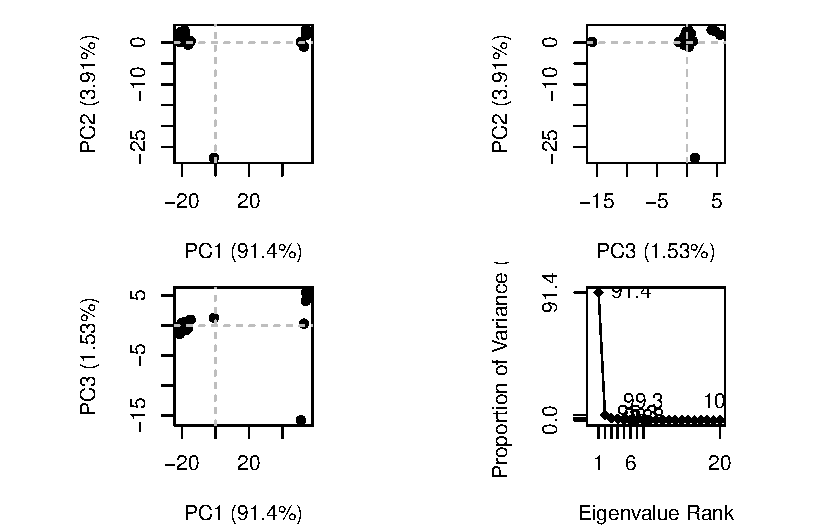
\includegraphics{Class-10_files/figure-pdf/unnamed-chunk-21-1.pdf}

\begin{Shaded}
\begin{Highlighting}[]
\FunctionTok{plot}\NormalTok{(pc.xray, }\DecValTok{1}\SpecialCharTok{:}\DecValTok{2}\NormalTok{)}
\end{Highlighting}
\end{Shaded}

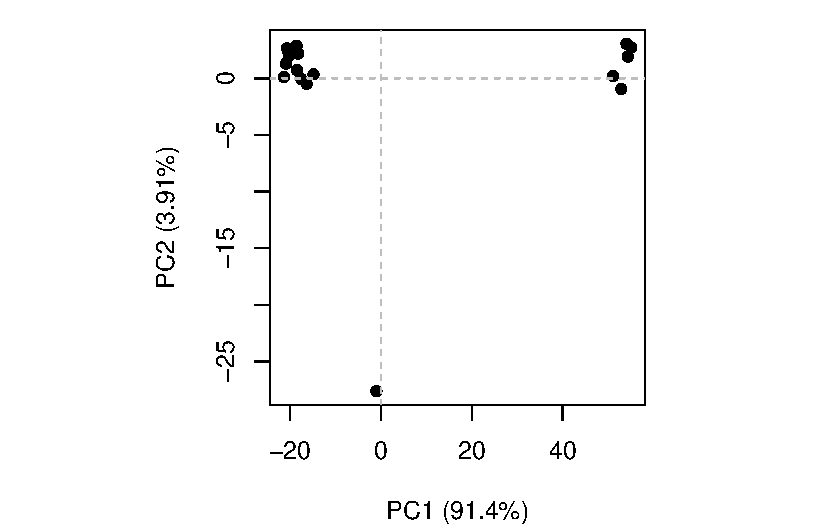
\includegraphics{Class-10_files/figure-pdf/unnamed-chunk-22-1.pdf}




\end{document}
